\newcommand{\zscene}{\bz^{\text{scene}}}
\newcommand{\zcamera}{\bz^{\text{cam}}}

\section{Method}%
\label{sec:method}

\method builds on the original VGGT, improving it in several ways.
We begin by describing the new architecture (\cref{sec:architecture}) and training pipeline (\cref{sec:training-losses}) of \method.
Then, we introduce a self-supervised training protocol to exploit unlabeled data (\cref{sec:self-supervised-training}) and a new data pipeline for robustly annotating millions of videos (\cref{sec:data}).

\subsection{A New Scalable Architecture}%
\label{sec:architecture}

\method, illustrated in \cref{fig:architecture}, is a feed-forward transformer $f$ that maps $N$ input images
$
I_1,\dots,I_N \in \mathbb{R}^{3\times H \times W}
$
to corresponding cameras and depth maps:
$$
((\bg_1, D_1),\dots,(\bg_N,D_N))
=
f(I_1,\dots,I_N),
$$
where
$D_i \in \mathbb{R}^{H \times W}$
is the depth map of image $I_i$ and
$\bg_i = (\bq_i, \bt_i, \bbf_i) \in \mathbb{R}^{9}$
is the concatenation of
the {rotation} quaternion $\bq_i \in \R^4$,
the {translation} vector $\bt_i \in \R^3$,
and the {field of view} $\bbf_i \in \R^2$
describing the corresponding camera.
As is commonly done~\cite{schonberger16structure-from-motion,wang24vggsfm:,wang25vggt}, we assume that the principal point is at the center of the image.
The problem formulation is thus similar to VGGT~\cite{wang25vggt}, except that the model \emph{does not} predict point maps or tracking features directly (although it still supervises them, as discussed in \cref{sec:training-losses}).
The network $f$ encodes each image into tokens (\cref{sec:feature-extraction-and-tokenization}), aggregates features across views with alternating-attention (\cref{sec:global-attention}), and maps the tokens to the final predictions using lightweight heads (\cref{sec:heads}).

\subsubsection{Feature Extraction and Tokenization}%
\label{sec:feature-extraction-and-tokenization}

We tokenize each image $I_i$ with a DINOv3-initialized vision transformer~\cite{simeoni25dinov3}, obtaining
$
\bz_i^F = \operatorname{DINO}(I_i) \in \mathbb{R}^{H'W'\times C}
$,
where $H'=H/r$ and $W'=W/r$ for patch size $r$.
For each image $I_i$, we also append one \emph{camera token} $\zcamera_i\in\mathbb{R}^{1\times C}$ and sixteen \emph{registers (scene tokens)} $\zscene_i\in\mathbb{R}^{16\times C}$.
The camera token is used to predict the camera parameters, and the registers aggregate information about the scene.
As in~\cite{wang25vggt}, these tokens can take one of two learnable parameters, one if image $I_i$ is the \emph{reference image} and the other otherwise.
These are then concatenated to form the set of tokens
$
\bz = (\bz_1,\dots,\bz_N) \in \mathbb{R}^{N \times (H'W'+17)\times C}
$
where $\bz_i = (\bz_i^F, \zcamera_i, \zscene_i)$ are the tokens of image $I_i$.

\subsubsection{Register Attention}%
\label{sec:global-attention}

\begin{figure}
\centering
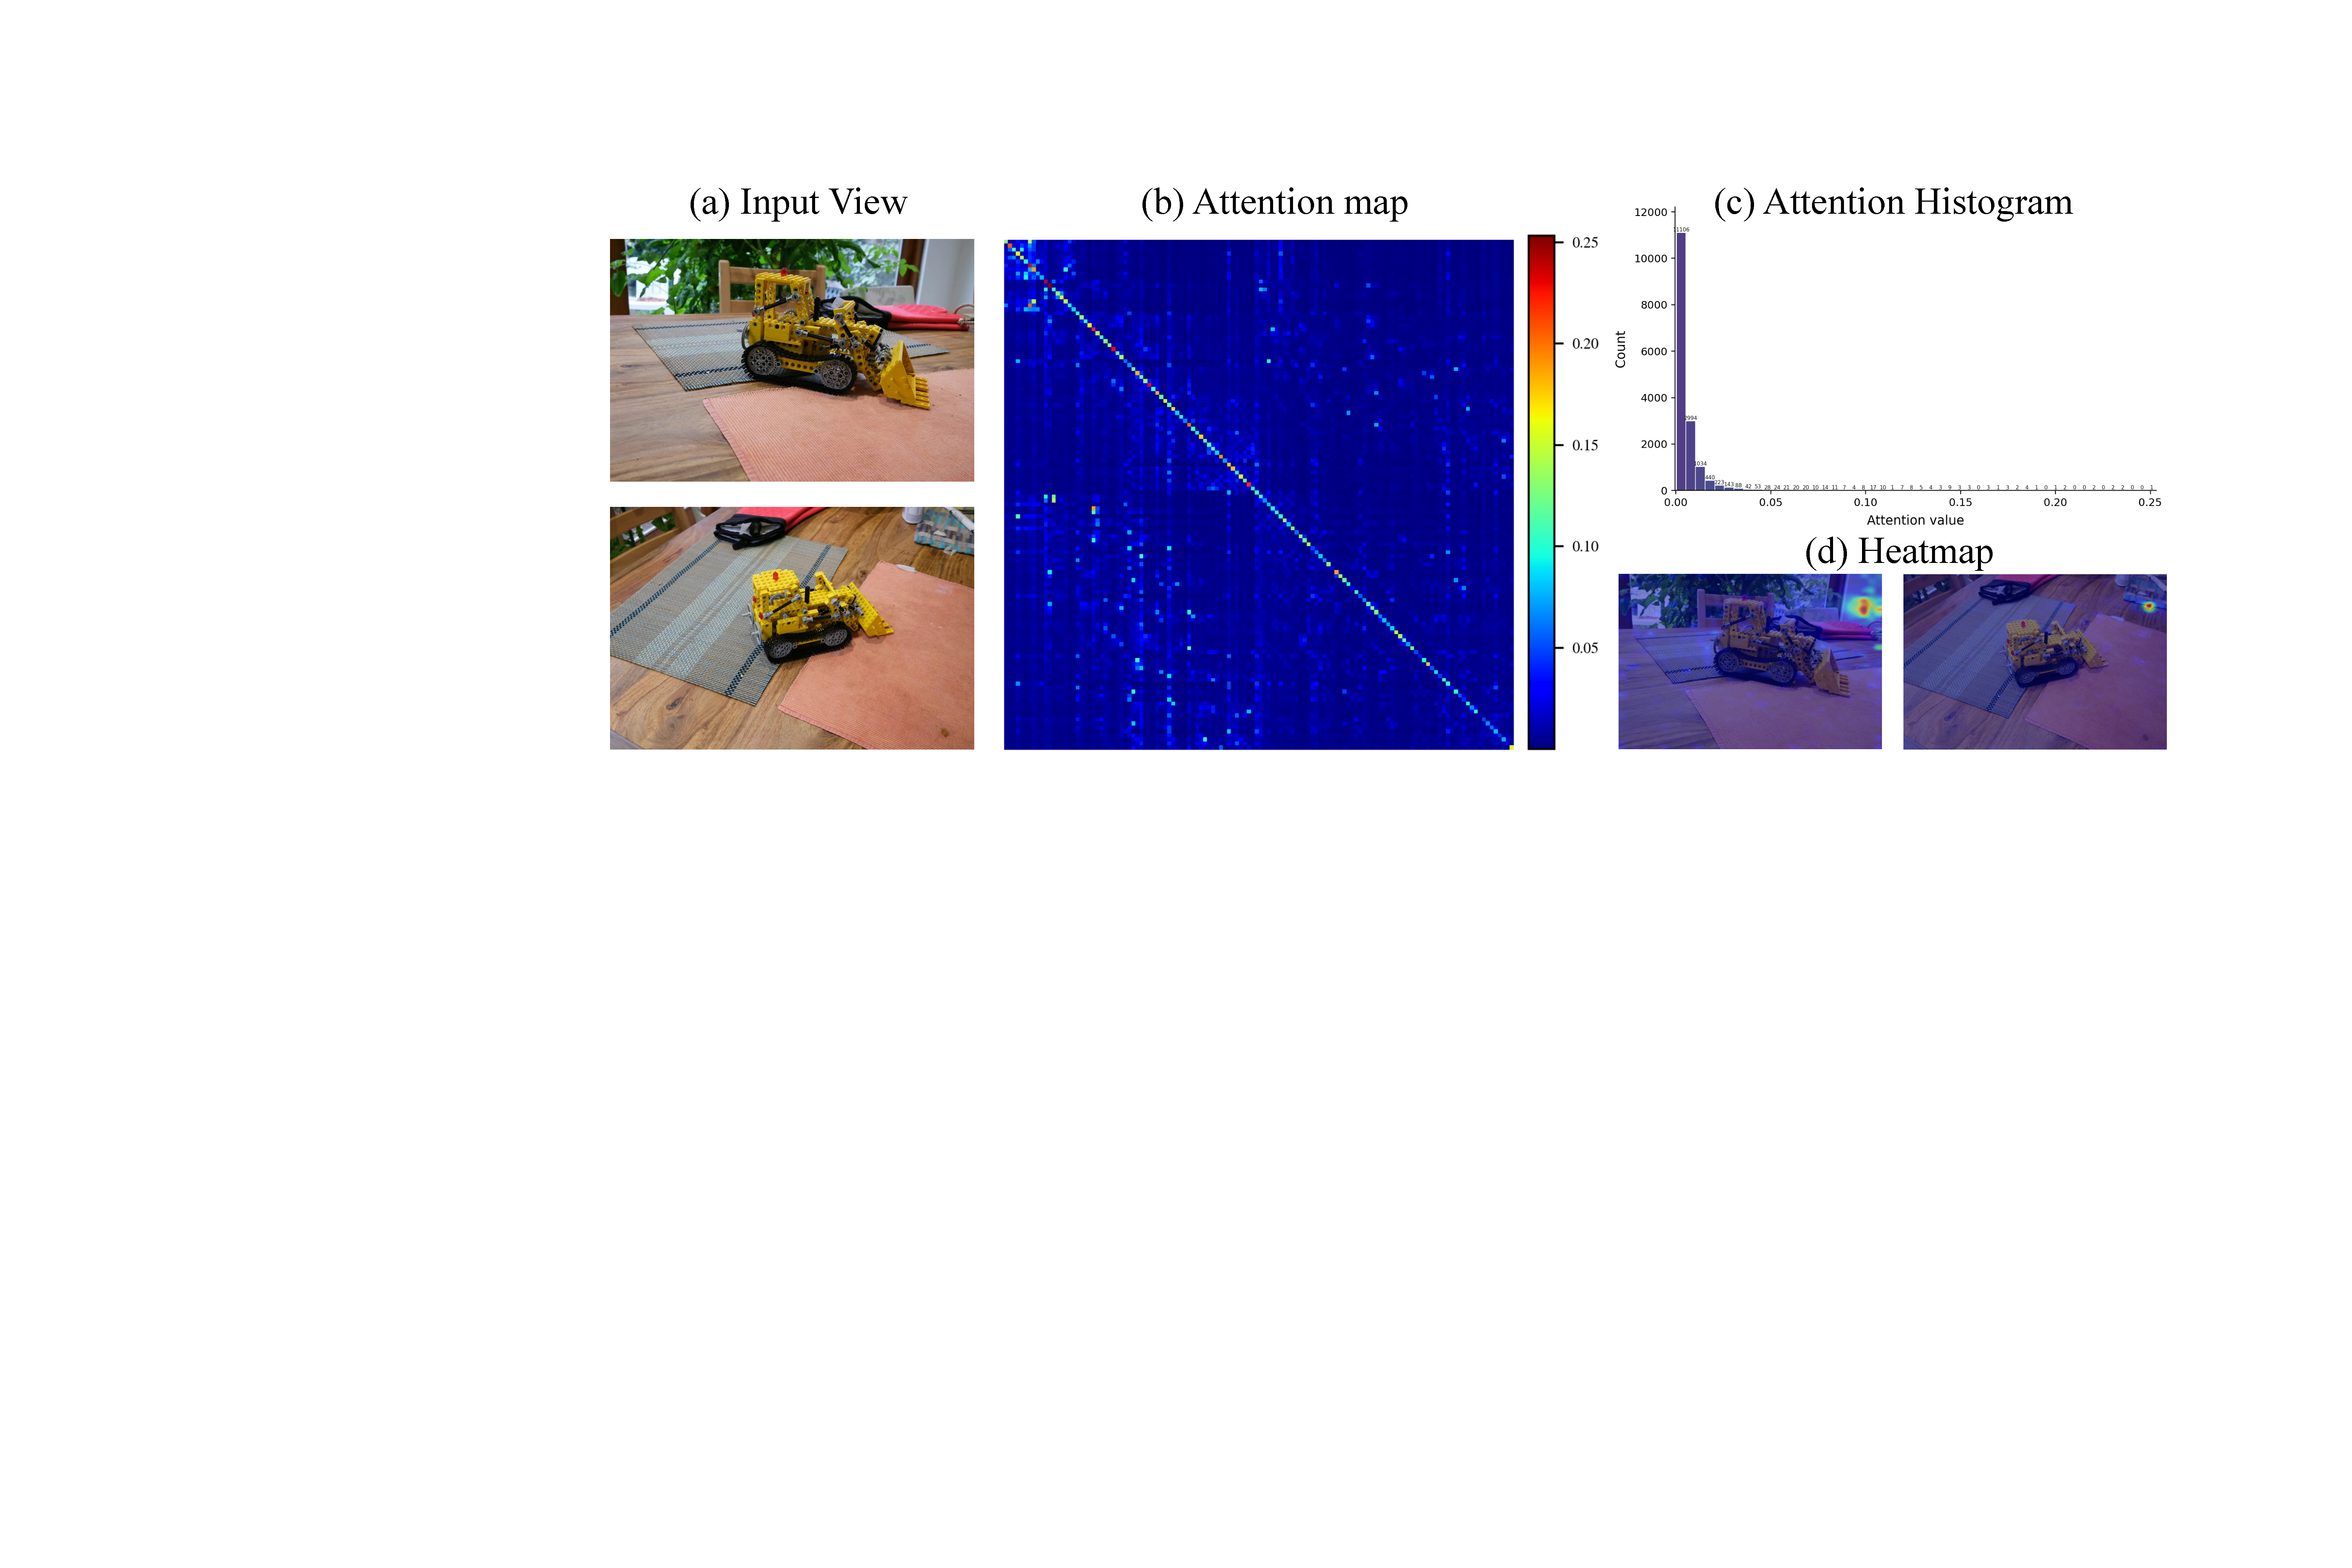
\includegraphics[width=0.98\linewidth]{figures/vgg_visualization.pdf}
\caption{\textbf{Visualization of Global Attention in VGGT}. As shown in (b) the global attention matrix, (c) its value distribution, and (d) spatial heatmaps, the attention in layer $13$ is quite sparse.}%
\label{fig:atten_visual}
\vspace{-8pt}
\end{figure}



\begin{figure*}
\centering
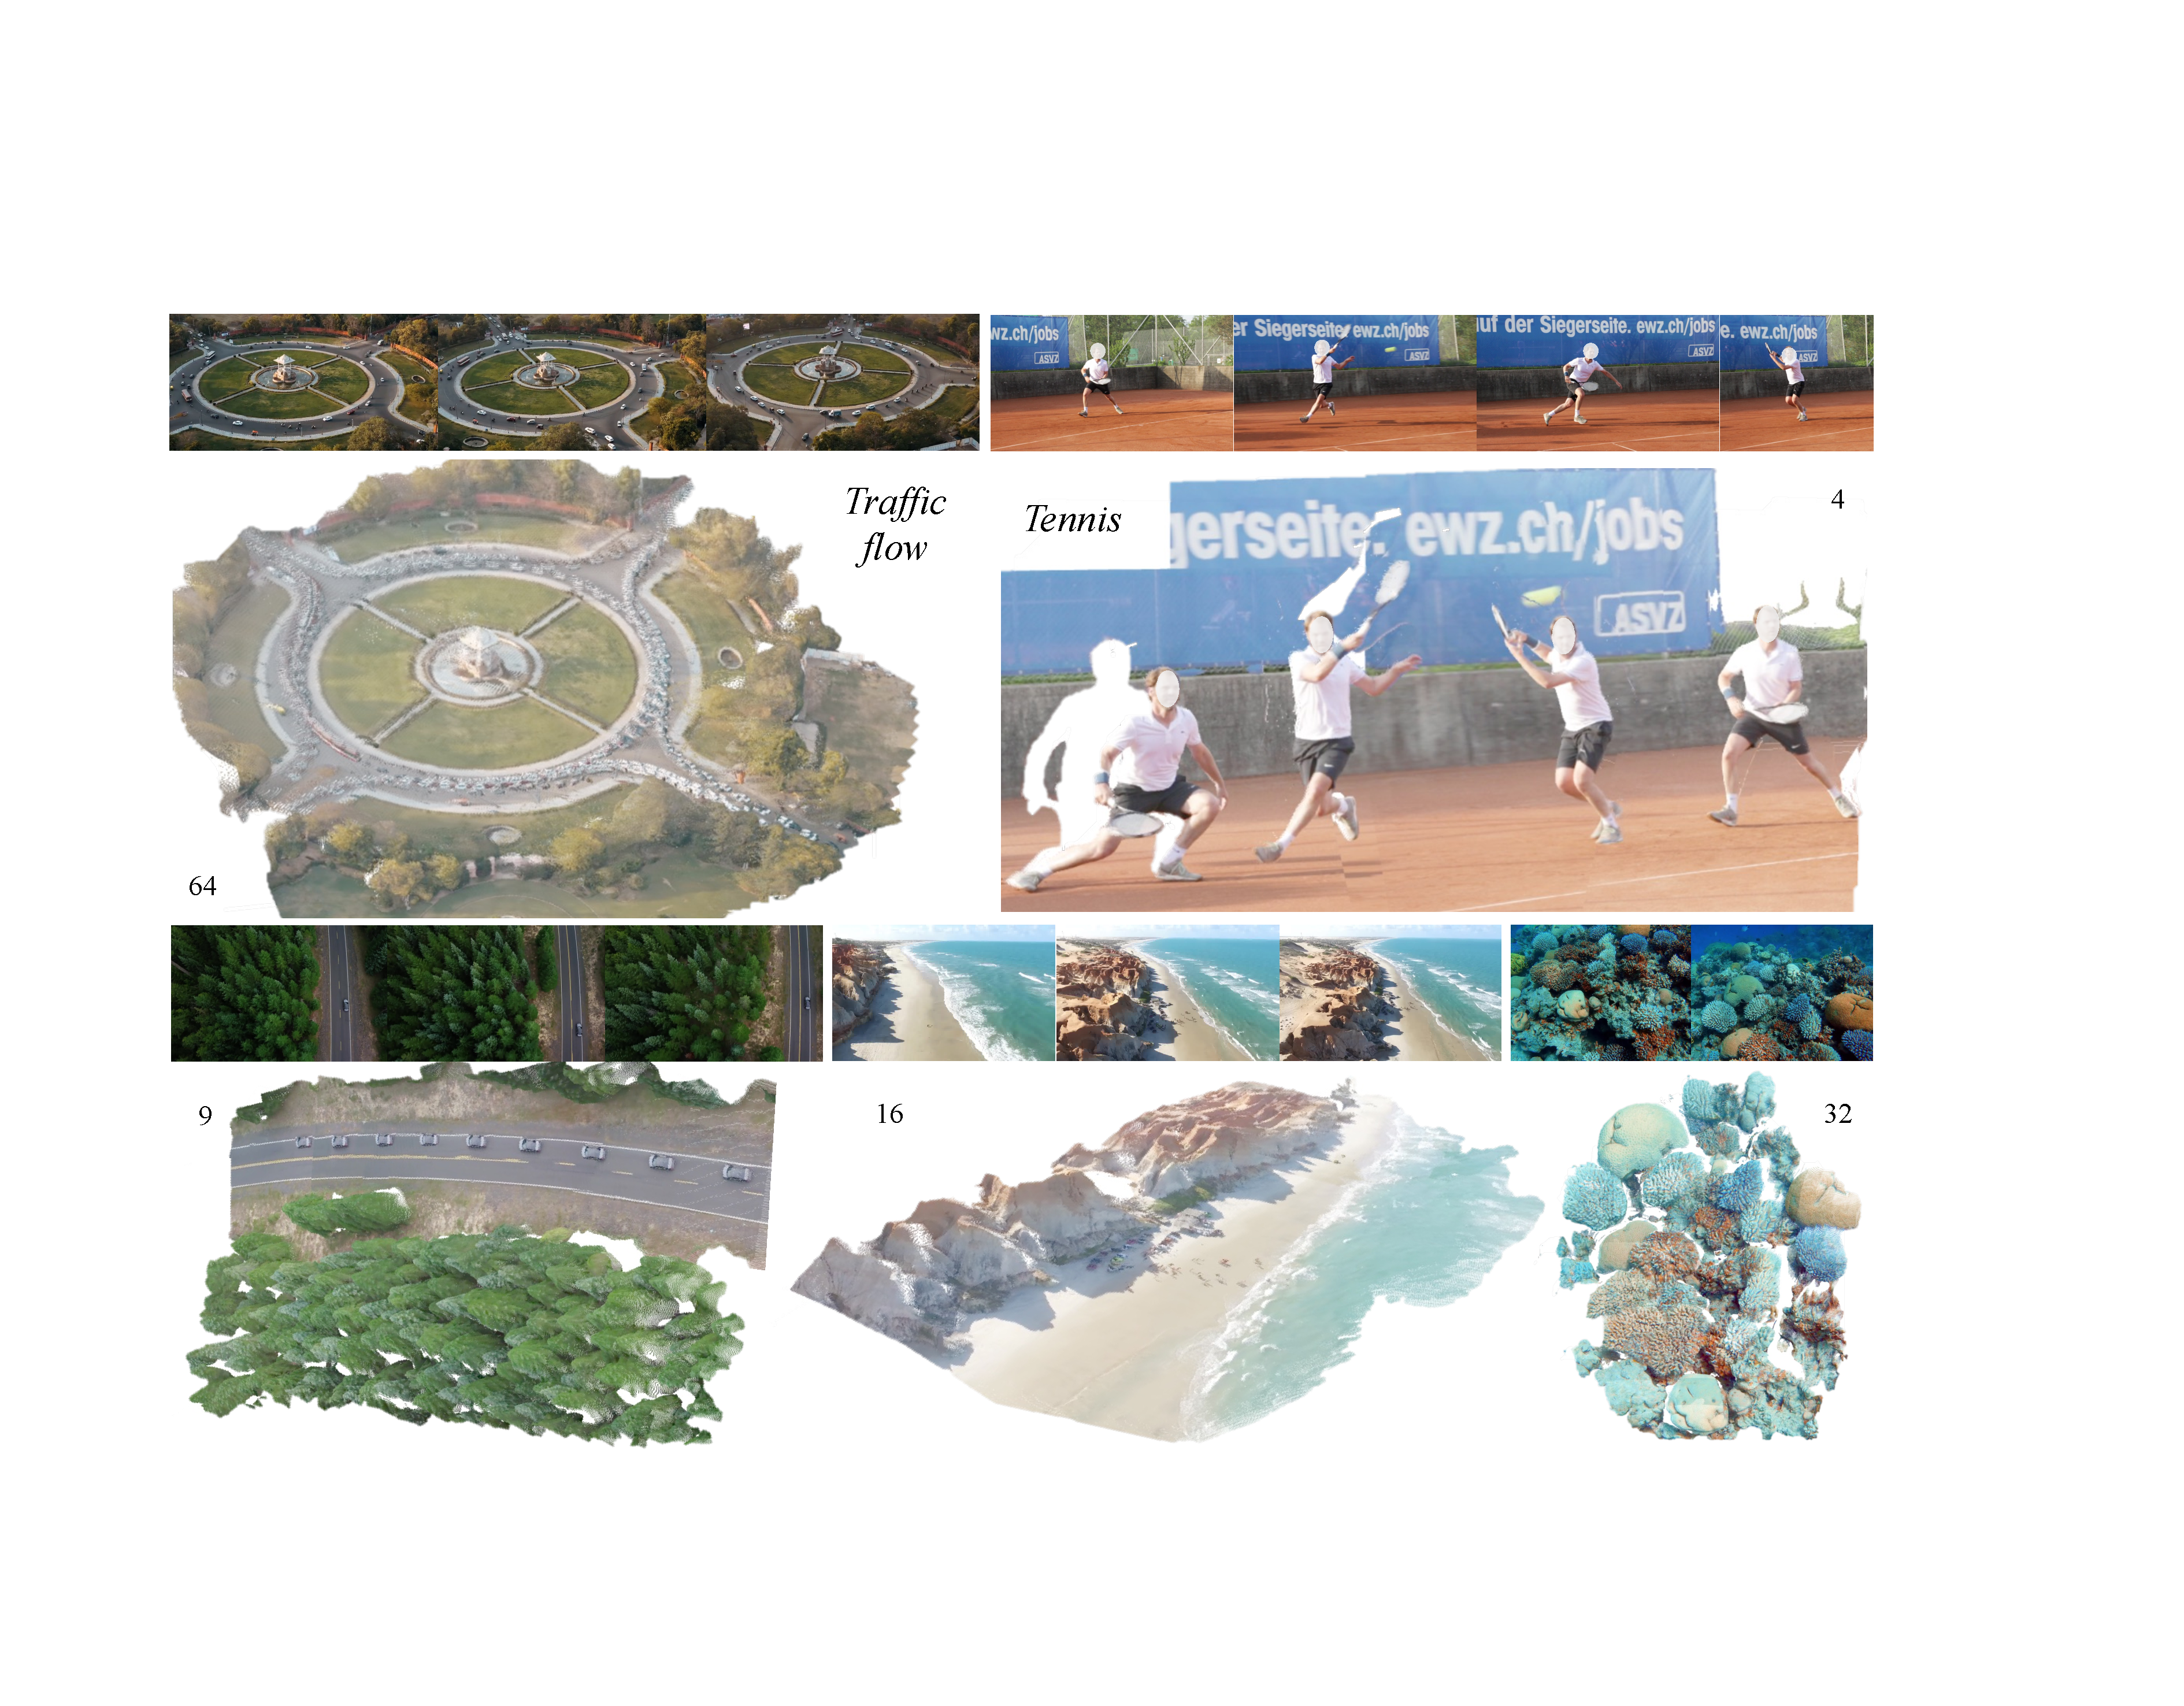
\includegraphics[width=\textwidth]{figures/qual_v6.pdf}
\caption{\textbf{Qualitative Results.} 
\method handles both static and dynamic content, as evidenced by the overlaid traffic flow and the tennis player's trajectory.
It also generalizes to hard scenes, \eg, underwater coral reefs.
Each example uses $64$, $4$, $9$, $16$, and $32$ input frames.
}%
\label{fig:qual}
\end{figure*}








Recall that VGGT uses \emph{alternating-attention}~\cite{wang25vggt}, interleaving between frame-wise self-attention within each image and global self-attention across all images, which are, by definition, permutation equivariant.
Frame-wise attention eliminates the need for frame-index embeddings, which would otherwise restrict the model's ability to generalize to a flexible number of input frames.
Therefore, none of the tokens has an explicit encoding of the corresponding image identity (except for indicating whether a frame is the reference).
{Global} attention is the standard attention layer applied to all tokens $\bz$, which we denote
$
\bz' = \operatorname{attn}(\bz)
$.
{Frame-wise} attention is similar, but applied independently to $\bz_i$ for each image $I_i$,
which we denote
$
\bz' =
\operatorname{attn}_f(\bz) =
(
    \operatorname{attn}(\bz_1), \dots,
    \operatorname{attn}(\bz_N)
)
$.
Global attention is where different frames interact, and thus where multi-frame scene information is formed.
At the same time, global attention is computationally expensive, as it attends to all tokens from all frames, with a cost that is quadratic in the total number of tokens.
Moreover, we observe that global attention maps are typically sparse, as shown in \cref{fig:atten_visual}, which may suggest that a small number of tokens are enough to exchange the corresponding information.
This is consistent with recent findings~\cite{shen26fastvggt:, wang25faster}.
We therefore replace 25\% of the global attention layers with \emph{register attention}, in which self-attention is restricted to the registers of all frames.
Formally, register attention updates only the registers:
$
\bz' = \operatorname{attn}_\text{scene}(\bz)
$
where
$
({\zscene_1}',\dots,{\zscene_N}') = \operatorname{attn}( \zscene_1,\dots,\zscene_N )
$,
\ie, only the registers participate in self-attention across frames in these blocks.
The updated registers then interact with each frame's image tokens in subsequent frame-wise attention blocks, redistributing the aggregated scene information back to the image tokens.
This encourages the final registers to carry global scene information, while also reducing the cost of global attention.

\subsubsection{Decoding}%
\label{sec:heads}

The final set of tokens $\bz' = (\bz_1',\dots,\bz_N')$ produced by the attention layers is decoded into depth maps and cameras.

\paragraph{Depth.}

In VGGT, all dense decoders are implemented with Dense Prediction Transformer (DPT) layers~\cite{ranftl21vision}.
However, the final convolutional blocks in these DPT heads maintain several high-resolution feature maps, which are memory-intensive.
To reduce this cost, we replace the blocks operating above $1/4$ of the input resolution with a lightweight upsampling head via a single MLP followed by a pixel-shuffle operator.
The MLP outputs $2u^{2}$ channels ($u=4$ in our implementation), and the pixel-shuffle operator rearranges them from $(H' \times W', 2u^{2})$ to $(uH') \times (uW') \times 2$, where the two output channels correspond to depth and confidence.

We also explored a fully convolution-free decoder that maps tokens to dense predictions using MLPs only.
While this works well on benchmarks, qualitatively it produces blocky artifacts in the predicted depth map, especially for outdoor scenes with distant structures such as sky or mountains, where depth is unbounded and thus not well-defined.
As such, we retain the early low-resolution convolutional layers in DPT since they are computationally inexpensive.

\paragraph{Camera.}

The cameras $(\bg_1,\dots,\bg_N)$ are predicted jointly by applying a lightweight transformer to the camera tokens and registers $\{(\zcamera_i,\zscene_i)\}_{i=1}^N$, followed by an MLP on each updated camera token.
Unlike VGGT, our camera head predicts camera parameters in a single pass, without iterative refinement.

\subsection{Training Losses}%
\label{sec:training-losses}

In VGGT, we found it beneficial to predict redundant dense heads (\eg, point maps and tracks), but doing so is expensive during training.
Instead, \method contains a single dense head for depth prediction.
Although the model does not \emph{directly} predict point maps and tracks, we \emph{still} supervise these quantities through corresponding losses.
We found this yields nearly the same performance as using multiple dense prediction heads while saving a significant amount of memory.
We thus optimize the loss:
{\small
\begin{equation}
\label{eq:training-loss}
\mathcal{L} =
\lambda_{\text{cam}}   \mathcal{L}_{\text{cam}} +
\lambda_{\text{depth}} \mathcal{L}_{\text{depth}} +
\lambda_{\text{point}} \mathcal{L}_{\text{point}} +
\lambda_{\text{match}} \mathcal{L}_{\text{match}}
\end{equation}}%
where $\lambda_{\text{cam}}$, $\lambda_{\text{depth}}$, $\lambda_{\text{point}}$, and $\lambda_{\text{match}}$ are weights.

\paragraph{Camera loss.}

The camera loss
$
\mathcal{L}_\text{cam} =
\sum_{i=1}^N \left| \hat{\bg}_i - \bg_i \right|
$
compares the predicted cameras $\hat{\bg}_i$ to the ground-truth ones $\bg_i$ using an $\ell_1$ objective, which we found to be more stable than the Huber loss used in VGGT\@.

\paragraph{Depth loss.}

Following VGGT, the depth loss uses aleatoric uncertainty and a gradient consistency term.
Additionally, we account for the relative scale with respect to the ground truth.
Therefore, we have:
$
\mathcal{L}_{\text{depth}} =
\sum_{i=1}^{N}
\left[
\left \|
c_i^{D} \odot \left( 1 + D_i^{-1} \right) \odot e_i \right \|
+
\left \| c_i^{D} \odot \nabla e_i \right \|
\right] - \alpha \sum_{i=1}^{N} \log c_i^{D}
$, where $e_i = \hat{D}_i - D_i$,  $c_i^{D}$ is the predicted uncertainty map, and $\odot$ denotes element-wise product.

\paragraph{Point loss.}

Point maps assign to each pixel the coordinates of the corresponding 3D point in the frame of the reference camera.
The point maps can thus be inferred from the depth maps and the camera parameters via unprojection.
Accordingly, our point loss $\mathcal{L}_{\text{point}}$ is the same as the depth loss $\mathcal{L}_{\text{depth}}$ up to replacing the residuals with
$
e_i = \pi^{-1}(\hat{D}_i, \hat{\bg}_i) - P_i
$,
where $\pi^{-1}$ denotes unprojection and $P_i$ is a point map.

\paragraph{Matching loss.}

The matching loss $\mathcal{L}_{\text{match}}$ is applied to the tokens output by the last attention layer.
It pulls together features of positive token pairs (corresponding to the same 3D location) and pushes apart negative pairs:
$
\mathcal{L}_{\text{match}} = \mathbb{E}_{\text{pos}}\!\big[-\log \sigma(s)\big] + \mathbb{E}_{\text{neg}}\!\big[-\log(1-\sigma(s))\big]
$,
where $s$ is the cosine similarity between $\ell_2$-normalized tokens, $\sigma$ is the sigmoid function, and $\mathbb{E}$ denotes averaging over positive and negative pairs, \ie, a weighted binary cross-entropy.
Details of how to construct the pairs are provided in the supplement.

\subsection{Dynamic Reconstruction}%
\label{sec:dynamic-reconstruction}

\method supports reconstructing dynamic scenes, which, among other benefits, unlocks orders-of-magnitude more training data (since most videos contain motion).
Dynamic reconstruction requires a statistical prior that constrains movement.
Classical non-rigid structure from motion~\cite{bregler00recovering, dai14a-simple,taylor10non-rigid} imposes hand-designed low-rank or local-rigidity constraints, which can be brittle and limited in generality.
A data-driven model like \method has the potential to learn a better prior from data.
However, the output representation determines how camera motion and scene motion are coupled. 
In particular, some recent methods~\cite{wang24dust3r:} use point maps to represent the scene and recover camera parameters from them.
This works well for static scenes, but in dynamic scenes it requires either segmenting out moving pixels, as in MonST3R~\cite{zhang24monst3r:}, or introducing extensions such as dynamic point maps~\cite{sucar25dynamic,sucar26v-dpm}.
Another option is to predict depth and ray maps~\cite{lin25depth}.
However, ray maps add an expensive dense output and can entangle camera information with pixel-wise appearance changes.
For example, a stationary camera observing a dancer has large motion but fixed camera parameters.
Therefore, as stated above, we predict only depth maps and camera parameters, and avoid explicit dynamic outputs such as motion masks. 


\subsection{Self-supervised Training}%
\label{sec:self-supervised-training}

Inspired by common practice in 2D vision~\cite{he20momentum, caron21emerging,oquab24dinov2:, simeoni25dinov3}, we use a teacher-student strategy for self-supervised learning with unlabeled videos.
Specifically, we maintain a \emph{student} network that is updated by gradient descent and a \emph{teacher} network that is updated only via an exponential moving average of the student network.
Both networks are initialized from the \method checkpoint trained on supervised data.
Given a video sequence, we feed the same set of frames to both networks but apply independent stochastic augmentations, including color jittering and blurring, random $90^\circ$ rotations, random patch masking, and random frame reordering (which affects the selection of the reference frame).
After restoring both streams to a common order, we require the student to match the teacher in two ways.
An $\ell_2$ feature-matching loss aligns the student's tokens with the teacher's across multiple layers.
Regression losses supervise the camera and depth.
To prevent collapse, the camera and depth heads are \emph{frozen} during self-supervision.
The teacher's parameters are updated as $\theta^{\mathrm{T}} \leftarrow m\,\theta^{\mathrm{T}} + (1-m)\,\theta^{\mathrm{S}}$ instead of gradient descent.
This distillation scheme thus enforces invariance to appearance changes and frame order, enabling effective learning from millions of unlabeled videos.
